
\section{QGIS}
QGIS merupakan sebuah perangkat SIG Open Source yang user friendly dengan lisensi di General Public License. QGIS merupakan suatu proyek yang tidak resmi dari Open Source OSGeo. QGIS dapat dijalankan pada OS Linux, Unix, Windows, Android dan Mac OSX. serta mendukung banyak format dan fungsionalitas data dari vektor, basisdata dan raster.
Quantum GIS mendukung GPS tools untuk upload atau download data ke unit GPS. Pengguna juga bisa mengkonversi format GPS ke format GPX atau melakukan kegiatan import atau export data format GPX.
Jika pengguna mempunyai sebuah web server yang telah terpasang fitur UMN MapServer, pengguna dapat melakukan publikasi map di internet untuk berbagi dengan pengguna lainnya.

SIG adalah sebuah perangkat sistem yang dirancang untuk memungkinkan orang-orang bekerja dengan data yang berkaitan. SIG memungkinkan pembuatan, penyimpanan, manipulasi, dan analisis data geografis. SIG merupakan satu konsep yang dapat melibatkan hardware dan software yang rumit. Tetapi, untuk memenuhi tujuan kebanyakan orang, yang dibutuhkan adalah sebuah perangkat lunak SIG yang sederhana, dan pada unit ini kita akan mempelajari bagaimana menggunakan aplikasi open-source yang unggul, QGIS.

\subsection{Getting QGIS}
\begin{enumerate}
\item
Buka browser internet Anda dan ketikkan pada bagian atas jendela browser Anda dengan tulisan qgis.org. Kemudian tekan Enter.\ref{image1}.
\begin{figure}[ht]
        \centerline{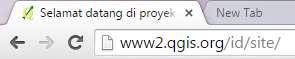
\includegraphics[width=0.25\textwidth]{figures/image1}}
        \caption{gambar}
        \label{image1}
        \end{figure}

Situs resmi QGIS akan terlihat seperti ini:\ref{image2}.
\begin{figure}[ht]
        \centerline{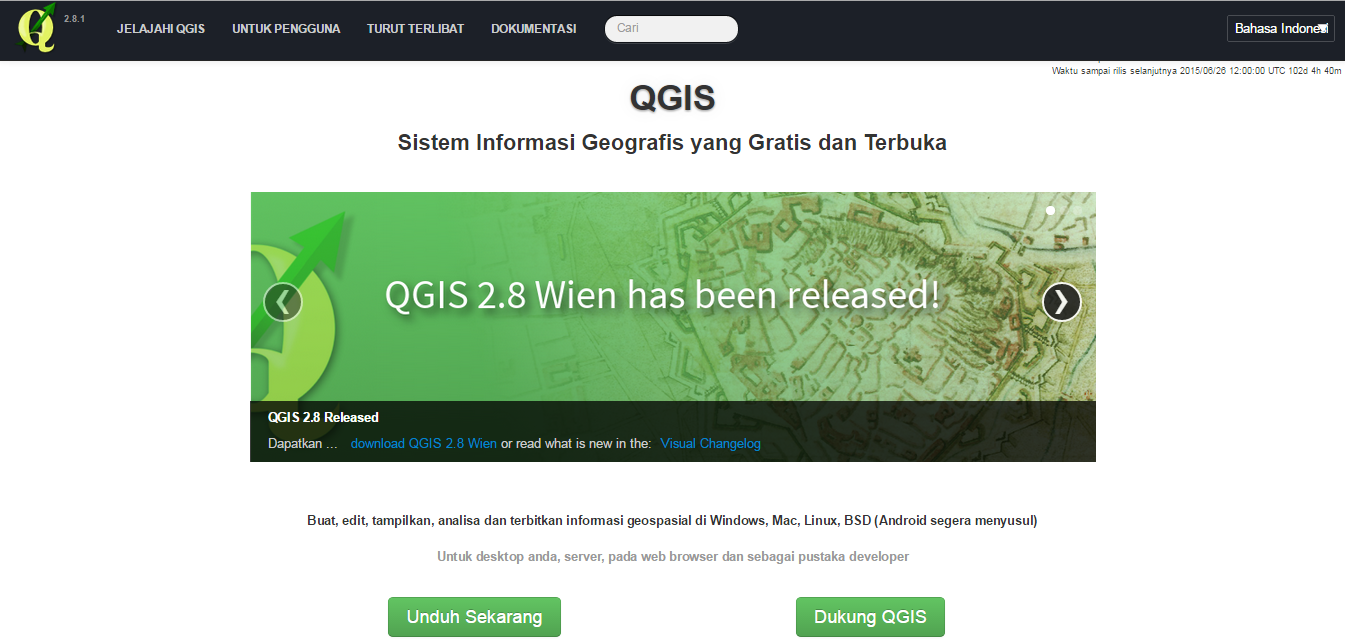
\includegraphics[width=1.00\textwidth]{figures/image2}}
        \caption{gambar}
        \label{image2}
        \end{figure}
\item
Klik Unduh Sekarang
\item
Jika Anda menggunakan Windows, klik pada QGIS Standalone Installer Version 2.8 (32 bit). Nomor versi komputer Anda mungkin berbeda.\ref{image3}.
\begin{figure}[ht]
        \centerline{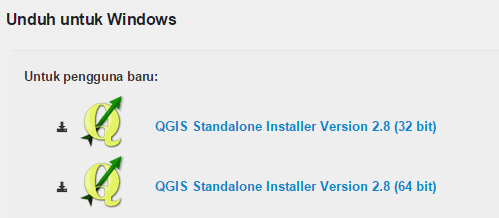
\includegraphics[width=0.25\textwidth]{figures/image3}}
        \caption{gambar}
        \label{image3}
        \end{figure}
\item
Jika Anda tidak menggunakan Windows, pilih Sistem Operasi Anda dari menu yang tersedia. Ikuti intruksi instalasi.\ref{image4}.
\begin{figure}[ht]
        \centerline{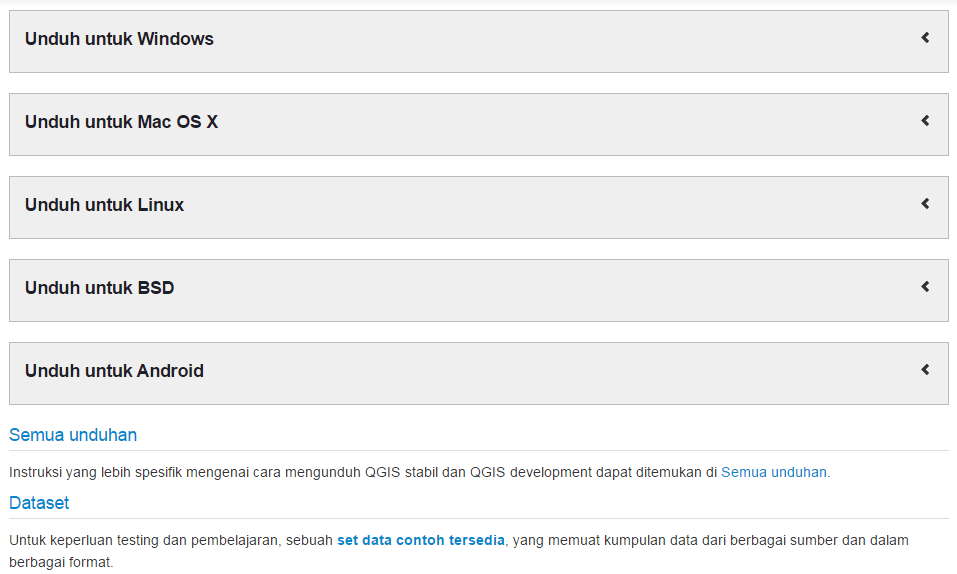
\includegraphics[width=0.25\textwidth]{figures/image4}}
        \caption{gambar}
        \label{image4}
        \end{figure}
\item
Ketika file selesai didownload, jalankan dan ikuti perintah untuk menginstal QGIS.
\end{enumerate}

\subsection{Installing QGIS}
\begin{enumerate}
\item
Buka folder dimana anda menyimpan file instalasi QGIS.\ref{image5}.
\begin{figure}[ht]
        \centerline{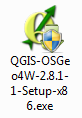
\includegraphics[width=0.05\textwidth]{figures/image5}}
        \caption{gambar}
        \label{image5}
        \end{figure}
\item
Jalankan file instalasi tersebut. Jika Anda menginstal QGIS versi 2.x, akan terlihat seperti ini:\ref{image6}.
\begin{figure}[ht]
        \centerline{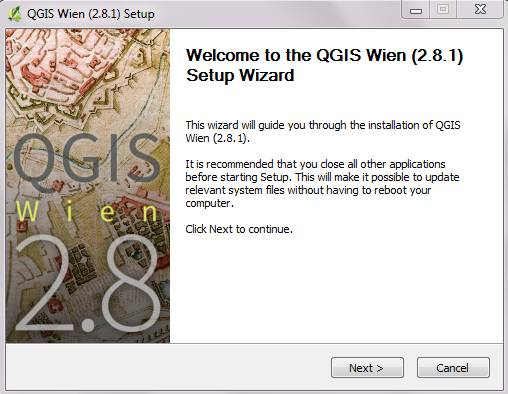
\includegraphics[width=0.25\textwidth]{figures/image6}}
        \caption{gambar}
        \label{image6}
        \end{figure}
\item 
Klik Next
\item
Klik I Agree untuk setuju dengan syarat dan ketentuan yang berlaku.\ref{image7}.
\begin{figure}[ht]
        \centerline{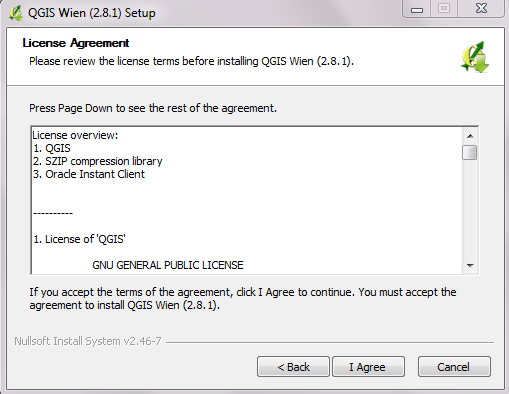
\includegraphics[width=0.25\textwidth]{figures/image7}}
        \caption{gambar}
        \label{image7}
        \end{figure}
\item
Pada jendela berikutnya Anda akan ditanyakan dimana Anda akan menginstall QGIS. Pada kasus umum, pengaturan bawaan yang ada sudah dapat digunakan. Klik Next.\ref{image8}.
\begin{figure}[ht]
        \centerline{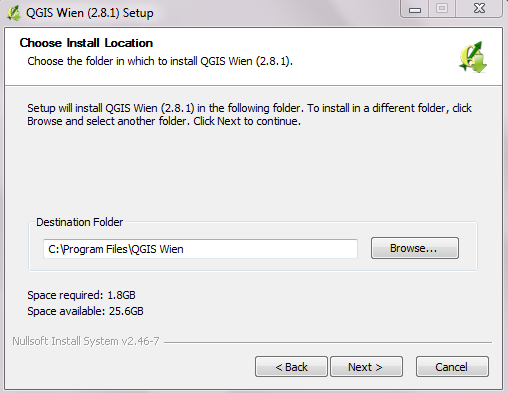
\includegraphics[width=0.25\textwidth]{figures/image8}}
        \caption{gambar}
        \label{image8}
        \end{figure}
\item
Pada jendela berikutnya, klik Install tanpa mencentang apapun yang ada di dalam kotak.\ref{image9}.
\begin{figure}[ht]
        \centerline{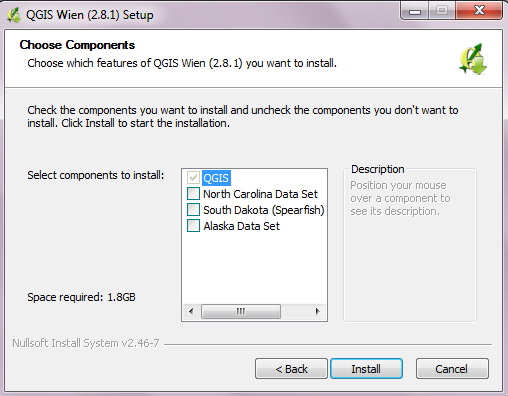
\includegraphics[width=0.25\textwidth]{figures/image9}}
        \caption{gambar}
        \label{image9}
        \end{figure}

QGIS akan memulai untuk menginstall. Ini mungkin akan membutuhkan beberapa waktu untuk selesai.\ref{image10}.
\begin{figure}[ht]
        \centerline{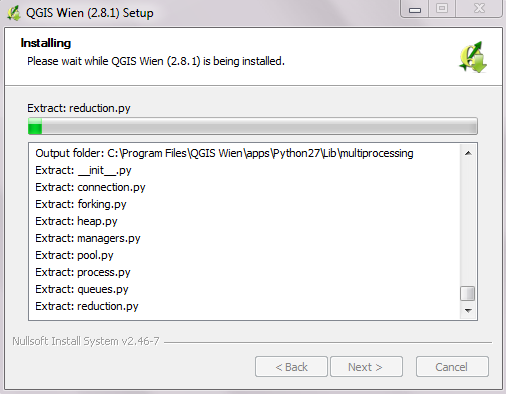
\includegraphics[width=0.25\textwidth]{figures/image10}}
        \caption{gambar}
        \label{image10}
        \end{figure}
\item
Klik Finish untuk melengkapi instalasi. Kemudian komputer Anda akan me-reboot secara otomatis.\ref{image11}.
\begin{figure}[ht]
        \centerline{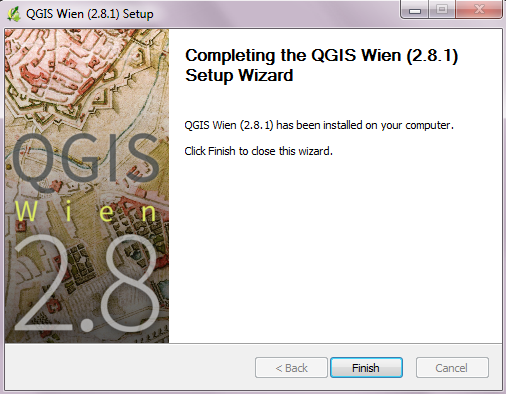
\includegraphics[width=0.25\textwidth]{figures/image11}}
        \caption{gambar}
        \label{image11}
        \end{figure}
\item
Buka QGIS dari Start Menu, berikut tampilan QGIS.\ref{image12}.
\begin{figure}[ht]
        \centerline{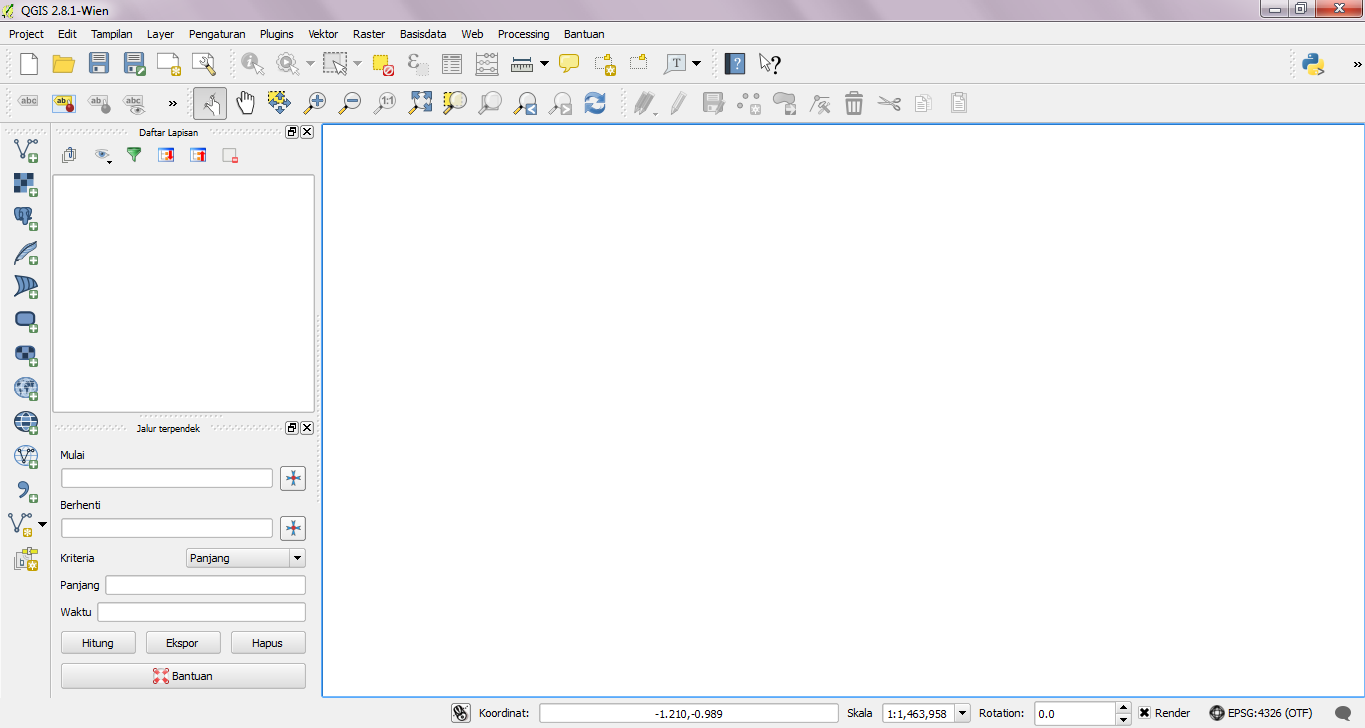
\includegraphics[width=0.25\textwidth]{figures/image12}}
        \caption{gambar}
        \label{image12}
        \end{figure}
\end{enumerate}

\subsection{Classification}
Pemberian label merupakan cara untuk mengkomunikasikan informasi seperti nama dari suatu tempat. Contohnya kita ingin menunjukkan tiap-tiap jenis vegetasi tersebut berada dimana. Dengan menggunakan sebuah label, akan tampak seperti gambar ini:\ref{image13}.
\begin{figure}[ht]
        \centerline{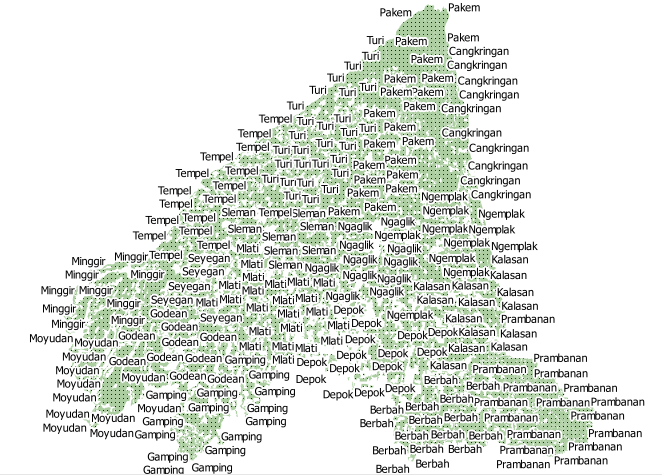
\includegraphics[width=0.25\textwidth]{figures/image13}}
        \caption{gambar}
        \label{image13}
        \end{figure}
Bisa kita lihat, hal tersebut tampak tidak ideal, jadi kita membutuhkan solusi yang lain. 


\subsection{Toolbar}
Pada bagian atas dari tampilan QGIS terdapat banyak sekali tool, dimana masing-masing tool tersebut masuk ke dalam beberapa kategori “toolbar”. Misalnya file mengizinkan pengguna untuk menyimpan dan memulai proyek baru.\ref{toolbar}
\begin{figure}[ht]
    \centerline{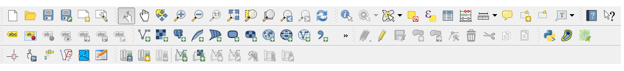
\includegraphics[width=0.25\textwidth]{figures/toolbar}}
    \caption{gambar toolbar yang ada pada QGis}
    \label{toolbar}
    \end{figure}

Dengan mengarakan mouse ke ikon, nama pada tool akan muncul untuk membantu mengidentifikasi setiap tool yang ada. Tool dikelompokkan sesuai fungsi pada toolbars. dengan meng-klik menggunakan mouse ,dapat memindahkan toolbar ke tempat yang lebih sesuai.\ref{toolbar1}.
\begin{figure}[ht]
    \centerline{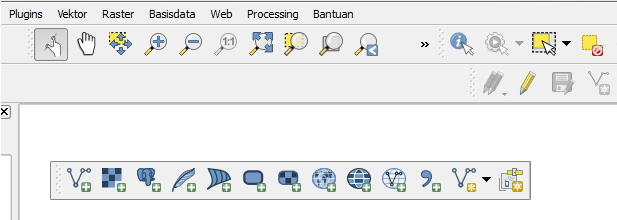
\includegraphics[width=0.25\textwidth]{figures/toolbar1}}
    \caption{gambar toolbar yang ada pada QGis}
    \label{toolbar1}
    \end{figure}
    
\subsection{Status Bar}
Status bar akan menampilkan informasi mengenai peta Anda. pengguna juga diperbolehkan untuk mengatur skala pada peta dan melihat koordinat peta.

Koordinat peta ini sama dengan tipe koordinat yang telah Anda pelajari ketika Anda belajar mengenai GPS.
Mungkin hal ini masih belum terlalu jelas untuk Anda, tapi seiring dengan meningkatnya kemampuan Anda di SIG, hal ini nantinya akan terlihat masuk akal. \ref{statbar}.
\begin{figure}[ht]
    \centerline{
\includegraphics[width=0.25\textwidth]{figures/statbar}}
    \caption{gambar status bar yang ada pada QGis}
    \label{statbar}
    \end{figure}

\subsection{Menu Bar}
Menu bar memberikan akses ke berbagai fitur QGIS menggunakan hirarki menu standar. Menu utama dan beberapa pilihan menu yang tercantum dengan ikon yang sesuai seperti yang ditampilkan pada toolbar dibawah ini. serta cara pintas keyboard. Cara pintas keyboard juga dapat dikonfigurasi secara manual (cara pintas yang disajikan dalam bagian ini adalah default), menggunakan [Configure Shortcuts] alat di bawah Setting. Beberapa pilihan menu hanya muncul jika plugin yang sesuai dimuat. Untuk informasi lebih lanjut tentang alat dan toolbar, lihat Bagian Toolbar. \ref{menubar}
\begin{enumerate}
\item
Project
\begin{figure}[ht]
    \centerline{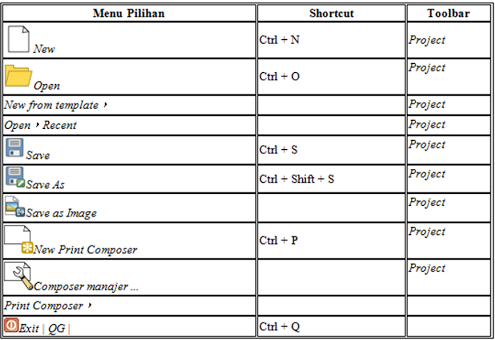
\includegraphics[width=0.25\textwidth]{figures/menubar}}
    \caption{Gambar project pada Menu Bar}
    \label{menubar}
    \end{figure}
\item
Edit
\begin{figure}[ht]
    \centerline{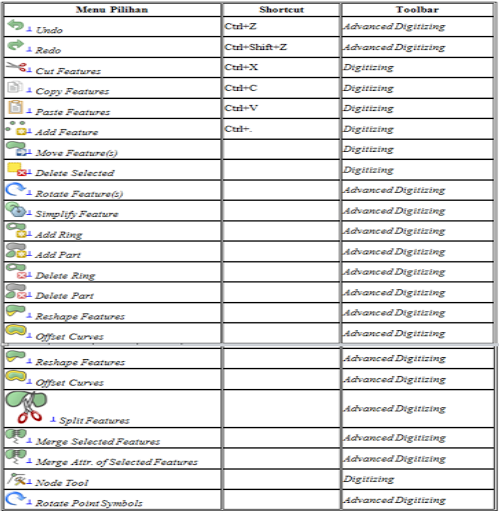
\includegraphics[width=0.25\textwidth]{figures/menubar1}}
    \caption{Gambar edit pada Menu Bar}
    \label{menubar1}
    \end{figure}
\item
View
\begin{figure}[ht]
    \centerline{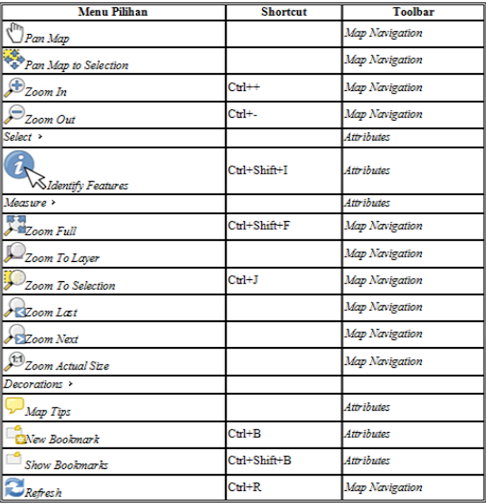
\includegraphics[width=0.25\textwidth]{figures/menubar2}}
    \caption{Gambar view pada Menu Bar}
    \label{menubar2}
    \end{figure}
\item
Setting
\begin{figure}[ht]
    \centerline{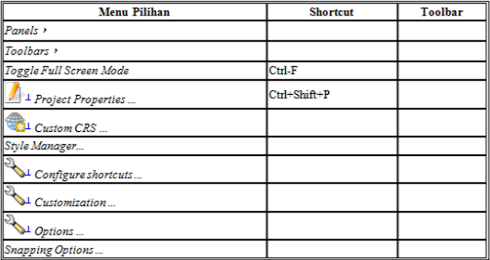
\includegraphics[width=0.25\textwidth]{figures/menubar3}}
    \caption{Gambar setting pada Menu Bar}
    \label{menubar3}
    \end{figure}
\item
Plugin
\begin{figure}[ht]
    \centerline{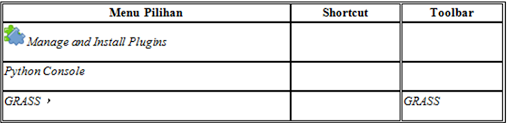
\includegraphics[width=0.25\textwidth]{figures/menubar4}}
    \caption{Gambar plugin pada Menu Bar}
    \label{menubar4}
    \end{figure}
\item
Vector
\begin{figure}[ht]
    \centerline{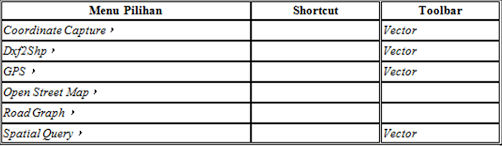
\includegraphics[width=0.25\textwidth]{figures/menubar5}}
    \caption{Gambar vector pada Menu Bar}
    \label{menubar5}
    \end{figure}
\item
Raster
\begin{figure}[ht]
    \centerline{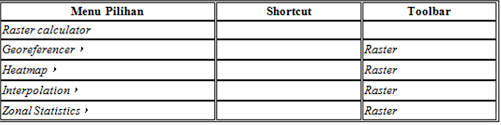
\includegraphics[width=0.25\textwidth]{figures/menubar6}}
    \caption{Gambar raster pada Menu Bar}
    \label{menubar6}
    \end{figure}
\item
Database
\begin{figure}[ht]
    \centerline{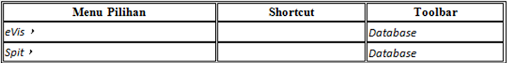
\includegraphics[width=0.25\textwidth]{figures/menubar7}}
    \caption{Gambar database pada Menu Bar}
    \label{menubar7}
    \end{figure}
\item
Pengolahan
\begin{figure}[ht]
    \centerline{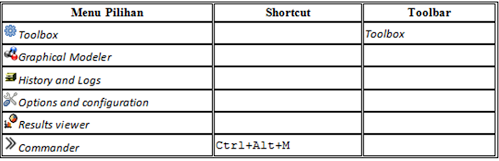
\includegraphics[width=0.25\textwidth]{figures/menubar8}}
    \caption{Gambar pengolahan pada Menu Bar}
    \label{menubar8}
    \end{figure}
\item
Bantuan
\begin{figure}[ht]
    \centerline{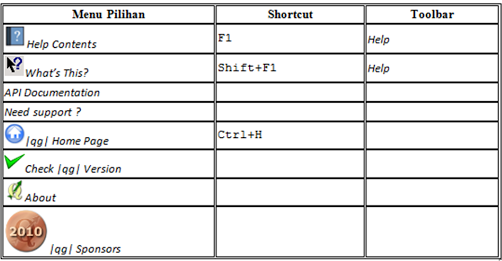
\includegraphics[width=0.25\textwidth]{figures/menubar9}}
    \caption{Gambar bantuan pada Menu Bar}
    \label{menubar9}
    \end{figure}
\end{enumerate}

\subsection{Atribut}
Data gis mempunyai fitur dan attribut. Atributt adalah data terstruktur mengenai setiap fitur. Cara ini menunjukkan bagaimana cara melakukan query standard pada attribut di QGIS.
Berikut langkahnya :
\begin{enumerate}
\item
Buka proyek yang telah dikerjakan sebelumnya.
\item
Pilih salah satu jalan pada panel daftar Layer.
\item
Klik kanan, dan klik tombol Open Attribute Table :
Akann terlihat tabel dengan data yang lebih banyak tentang layer jalan. Data ekstra tersebut disebut data atribut. Garis-garis yang Anda dapat lihat pada peta Anda menggambarkan kemana garis tersebut menuju – ini merupakan data spatial.
\item
Lihatlah pada tabel atribut. Setiap baris tabel menghubungkan satu fitur pada layer jalan. Setiap kolom mengandung satu atribut.
\item
Tutup tabel atribut
\end{enumerate}

\subsection{Label Tool}
Untuk menambahkan label pada QGIS ada beberapa cara lebih baik dibandingkan yang lain. Berikut langkah-langkahnya :\ref{label}
\begin{enumerate}
\item
Pergi ke menu item View --> Toolbars
\item
Pastikan item Label telah memiliki tanda centang disebelahnya. Jika belum, klik pada item Label dan fitur tersebut akan diaktifkan.\ref{label}.
\begin{figure}[ht]
    \centerline{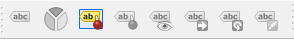
\includegraphics[width=0.25\textwidth]{figures/label}}
    \caption{Toolbar Label tampak seperti ini}
    \label{label}
    \end{figure}
\item
Klik layer POI\_Bandung\_OSM yang terdapat pada panel Daftar Layer, sehingga layer tersebut tersorot
\item
Klik tombol Layer Labelling Options
\begin{figure}[ht]
    \centerline{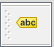
\includegraphics[width=0.25\textwidth]{figures/layer}}
    \caption{tombol Layer Labelling Options}
    \label{layer}
    \end{figure}
\item
Setelah klik tombol diatas maka akan muncul halaman pengaturan Layer Labelling. Centang kotak yang ada tulisan Layer this Label With
\begin{figure}[ht]
    \centerline{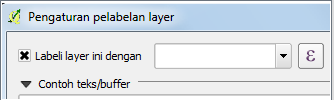
\includegraphics[width=0.25\textwidth]{figures/laylabel}}
    \caption{tombol Layer this Label With}
    \label{laylabel}
    \end{figure}
\item
Pilih Field Name untuk pemberian label
\begin{figure}[ht]
    \centerline{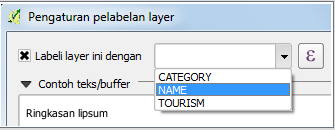
\includegraphics[width=0.25\textwidth]{figures/name}}
    \caption{Field Name}
    \label{name}
    \end{figure}
\item
Klik OK maka peta akan muncul dengan label
\end{enumerate}

\subsection{Fitur Dasar Quantum GIS Dalam Pengelolaan Data Vektor dan Raster}
Sebagai perangkat lunak Sistem Informasi Geografik, Quantum GIS memiliki kapabilitas untuk menampilkan, mengolah dan menyajikan data. Contohnya sebagai berikut:
\begin{enumerate}
\item
Membaca dan mengedit data dalam format vektor dan raster, termasuk data atribut
Quantum GIS dapat membaca dan mengolah data dalam banyak format, baik dalam bentuk raster maupun vektor.
\item
Konversi sistem koordinat dan proyeksi peta
Konversi sistem koordinat dan proyeksi peta dapat dilakukan dengan mudah di Quantum GIS, dengan memilih opsi CRS ketika menyimpan data, seperti gambar berikut:
\begin{figure}[ht]
    \centerline{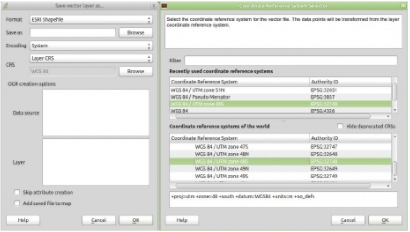
\includegraphics[width=0.25\textwidth]{figures/proyeksi}}
    \caption{Gambar konversi sistem koordinat dan proyeksi peta pada QGIS}
    \label{proyeksi}
    \end{figure}
\item
Navigasi peta
Pada Quantum GIS, navigasi peta bisa dilakukan melalui toolbar khusus, dengan fungsi navigasi yang bisa digunakan antara lain: Perbesar (zoom in) dan Perkecil (zoom out), Penggeseran (pan).
\item
Setting tampilan peta
Tampilan peta dapat diatur melalui menu Layer > Properties. Hal-hal yang dapat diatur antara lain: warna dan pola arsiran, warna dan ketebalan garis, bentuk dan ukuran simbol, dan sebagainya. Tampilan setting layer seperti berikut:
\begin{figure}[ht]
    \centerline{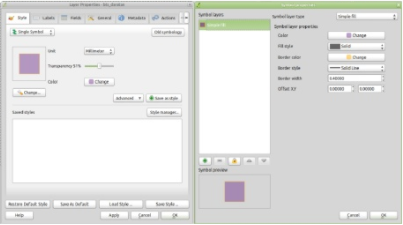
\includegraphics[width=0.25\textwidth]{figures/setting}}
    \caption{Gambar setting tampilan peta pada QGIS}
    \label{setting}
    \end{figure}
\end{enumerate}

\subsection{Menambahkan Data Vektor}
\begin{enumerate}
\item 
Buka proyek QGIS yang baru. Peta dan daftar layer yang akan tampak masih kosong.
\item
Terdapat dua cara untuk menambahkan sebuah layer vektor baru pada proyek.
\item
Klik pada tombol Navigasi ke direktori qgis/sarijadi/ dan pilih Jalan\_Sarijadi\_OSM, POI\_Sarijadi dan Kecamatan\_Sukasari. Anda dapat memilih lebih dari satu file dengan menahan tombol CTRL pada keyboard dan klik tiap file. Klik Open lalu Open lagi.
\end{enumerate}

Peta Anda sekarang akan terlihat seperti ini:\ref{vektor}
\begin{enumerate}
\item
Project
\begin{figure}[ht]
    \centerline{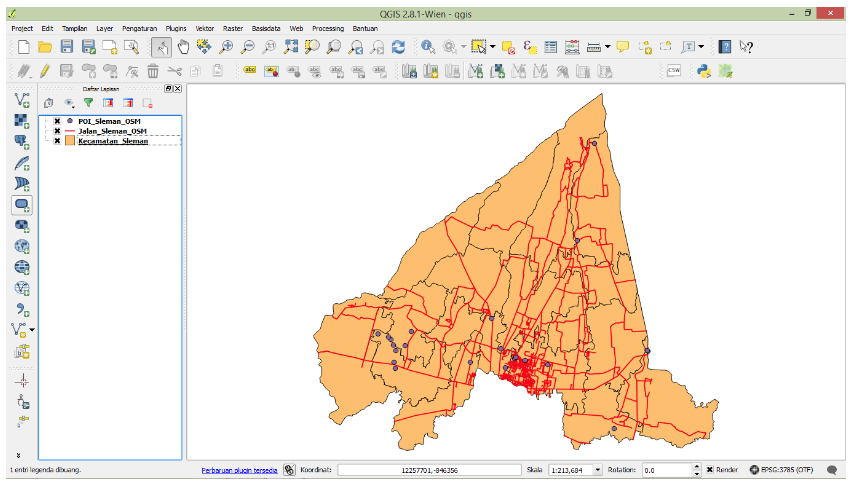
\includegraphics[width=0.25\textwidth]{figures/vektor}}
    \caption{Gambar vektor pada qgis}
    \label{vektor}
    \end{figure}

\end{enumerate}

\subsection{Mode Algoritma}
Pada mode algoritma ini menggunakan algoritma yang berbeda untuk memilah sebuah data ke kelas yang berbeda.
•	Interval sama: seperti namanya, metode ini akan menghasilkan kelas dengan ukuran yang sama.
•	Kuantil : Merupakan Metode untuk memutuskan kelas di mana jumlah nilai pada setiap kelas adalah sama.

\subsection{Klasifikasi Data Vektor}
Untuk menampilkan simbol-simbol yang berbeda pada sebuah objek. Contoh: Peta Kuliner, isinya objek yang telah diklasifikasikan berdasar jenis tempat kuliner.

\subsection{MS4W}
MapServer merupakan pengembangan sebuah perangkat lunak open source yang dapat digunakan untuk mengembangkan aplikasi internet-based yang melibatkan tampilan data spasial peta digital.\cite{supriantoaplikasi}

\begin{table}[h]
\caption{Paket dasar M4SW}
\centering
\begin{tabular}{cc}
\hline
1&Webserver Apache\\
\hline
2&PHP\\
\hline
3&MapServer CGI\\
\hline
4&PHP/Mapscript\\
\hline
5&Program utiliti (pustaka) GDAL dan OGR\\
\hline
6&Program utiliti MapServer (shp2img, legend, scalebar, sortshp, sym2img, shptree, dan tile4ms)\\
\hline
7&Ekstensi OGR/PHP\\
\hline
8&OWTChart\\
\hline
\end{tabular}
\end{table}

